\chapter{Interest Rate Modelling (An Introduction)}\label{ch:interest-rate-modelling}

In previous chapters we introduced a simplified model for interest rates using a money market bank account in which interest accrues deterministically. In reality, interest rates are much more complex and evolve stochastically. At the end of 2021, as the global economy emerged from COVID-19, major economies had experienced nearly two years of near-zero, largely stationary interest rates that behaved almost deterministically.

As economies reopened in 2022, however, interest rates rose sharply and far more rapidly than market participants had anticipated, illustrating their fundamentally stochastic nature. In this chapter we introduce the largest segment of the global derivatives market: interest rate derivatives, along with an introduction to credit risk.

\section{The Bank Account Revisited}
Previously we treated the bank account as a deterministic process. We now allow the bank account to be stochastic. The bank account is a money market account accruing interest at the instantaneous \textbf{short rate} $r_t$. Its value at time $t$ is
\[
B_t = e^{\int_0^t r_s\dd s}, \qquad \dd B_t = r_t B_t\dd t.
\]
Although no Brownian increment appears explicitly in $\dd B_t$, the process $B_t$ is stochastic because $r_t$ is stochastic. We can therefore model $r_t$ directly; below we introduce three classical one-factor short-rate models.

\subsection*{Ho--Lee Model}
The Ho--Lee model is a simple one-factor model in which the short rate is driven by a single Brownian motion:
\[
\dd r_t = \theta_t\dd t + \sigma\dd W_t.
\]
Here $\theta_t$ represents the time-dependent drift of the short rate, which may be positive or negative to reflect rising or falling rate regimes. When $\theta_t \equiv 0$, interest rates fluctuate symmetrically around the initial level $r_0$.

The model is Gaussian, with
\begin{align*}
\E[r_T] &= r_0 + \int_0^T \theta_t\dd t, \\
\Var(r_T) &= \sigma^2 T.
\end{align*}

\subsection*{Ornstein--Uhlenbeck: Vasicek Model}
The Vasicek model introduces mean reversion into the short-rate dynamics:
\[
\dd r_t = \alpha(\theta - r_t)\dd t + \sigma\dd W_t,
\]
where $\alpha > 0$ is the speed of mean reversion, $\theta$ is the long-term mean of the short rate, and $\sigma > 0$ is the volatility of the short rate.

Solving this SDE is straightforward using the integrating factor $e^{\alpha t}$:
\begin{align*}
\dd r_t &= \alpha(\theta - r_t)\dd t + \sigma\dd W_t \\
\dd r_t + \alpha r_t\dd t &= \alpha\theta\dd t + \sigma\dd W_t \\
\dd(r_t e^{\alpha t}) &= \alpha\theta e^{\alpha t}\dd t + \sigma e^{\alpha t}\dd W_t \\
r_T e^{\alpha T} - r_0 &= \alpha\theta \int_0^T e^{\alpha t}\dd t + \sigma \int_0^T e^{\alpha t}\dd W_t \\
r_T e^{\alpha T} - r_0 &= \theta(e^{\alpha T} - 1) + \sigma \int_0^T e^{\alpha t}\dd W_t \\
r_T &= r_0 e^{-\alpha T} + \theta(1 - e^{-\alpha T}) + \sigma \int_0^T e^{-\alpha(T-t)}\dd W_t.
\end{align*}

Thus $r_T$ is Gaussian with
\begin{align*}
\E[r_T] &= r_0 e^{-\alpha T} + \theta(1 - e^{-\alpha T}), \\
\Var(r_T) &= \frac{\sigma^2}{2\alpha}\bigl(1 - e^{-2\alpha T}\bigr), \\
\lim_{T \to \infty} \E[r_T] &= \theta \qquad (\text{since } \alpha > 0).
\end{align*}

\subsection*{Ornstein--Uhlenbeck: Hull--White Model}
The Hull--White model extends Vasicek by allowing the model parameters to be time-dependent. Although $\alpha$ can also depend on time, in practice it is usually held constant ($\alpha > 0$):
\[
\dd r_t = \alpha(\theta_t - r_t)\dd t + \sigma_t\dd W_t.
\]
Repeating the integrating-factor derivation yields
\begin{align*}
r_T &= r_0 e^{-\alpha T} + \alpha \int_0^T \theta_t e^{-\alpha(T-t)}\dd t + \int_0^T \sigma_t e^{-\alpha(T-t)}\dd W_t, \\
\E[r_T] &= r_0 e^{-\alpha T} + \alpha \int_0^T \theta_t e^{-\alpha(T-t)}\dd t, \\
\Var(r_T) &= \int_0^T \sigma_t^2 e^{-2\alpha(T-t)}\dd t.
\end{align*}
Now $\lim_{T \to \infty} \E[r_T]$ depends on the asymptotic behavior of $\theta_t$.

All three models above are Gaussian, which implies that the integrated short rate $\int_0^T r_s\dd s$ is Gaussian and the money market account $B_T$ is log-normally distributed. While analytically tractable, Gaussian short-rate models assign positive probability to arbitrarily negative interest rates.

\subsection*{Cox--Ingersoll--Ross (CIR) Model}
To enforce non-negativity of interest rates while preserving mean reversion and analytical tractability, the \textbf{Cox--Ingersoll--Ross (CIR)} model introduces a square-root diffusion coefficient:
\begin{equation}\label{eq:cir-sde}
\dd r_t = \kappa(\theta - r_t)\dd t + \sigma\sqrt{r_t}\dd W_t,
\end{equation}
where $\kappa > 0$ is the speed of mean reversion, $\theta > 0$ is the long-term mean, and $\sigma > 0$ is the volatility parameter. As $r_t \downarrow 0$, the diffusion term $\sigma\sqrt{r_t}\dd W_t$ vanishes while the drift $\kappa\theta > 0$ pushes the rate back upward.

A classical boundary classification due to Feller determines whether the origin is attainable:
\begin{proposition}[Feller Condition]\label{prop:feller-condition}
    Suppose $r_0 > 0$ and $r_t$ satisfies \eqref{eq:cir-sde} with $\kappa, \theta, \sigma > 0$. If the \textbf{Feller condition}
    \[
    2\kappa\theta \geq \sigma^2
    \]
    holds, then the origin is inaccessible and $r_t > 0$ almost surely for all $t \geq 0$. If $0 < 2\kappa\theta < \sigma^2$, the process can reach $0$ with positive probability, after which it instantaneously reflects back into $(0, \infty)$.
\end{proposition}
\noindent\emph{Reference.} See W.~Feller (1951), \emph{Two Singular Diffusion Problems}, Annals of Mathematics 54(1), 173--182, and J.~C.~Cox, J.~E.~Ingersoll, and S.~A.~Ross (1985), \emph{A Theory of the Term Structure of Interest Rates}, Econometrica 53(2), 385--407.
Unlike the Vasicek model, $r_T$ in the CIR model is not Gaussian; instead, conditional on $r_0$, a suitably scaled multiple of $r_T$ follows a non-central chi-squared distribution with $\nu = 4\kappa\theta/\sigma^2$ degrees of freedom, mean $\E[r_T] = r_0 e^{-\kappa T} + \theta(1 - e^{-\kappa T})$, and variance
\[
\Var(r_T) = r_0 \frac{\sigma^2}{\kappa}\bigl(e^{-\kappa T} - e^{-2\kappa T}\bigr) + \frac{\theta\sigma^2}{2\kappa}\bigl(1 - e^{-\kappa T}\bigr)^2.
\]

\section{Tradable Interest Rate Assets (Bonds)}

Interest rates themselves are not tradable assets; they measure the cost of borrowing money. Unlike stocks, one cannot directly buy or sell an interest rate. Consequently, no-arbitrage pricing for interest rate derivatives requires introducing a tradable \textbf{interest rate asset}.

\begin{definition}\label{def:zcb}
    A \textbf{zero-coupon bond} (ZCB) with maturity $T$ is a contract that pays $1$ unit of currency at time $T$ and makes no intermediate payments. If the short rate were deterministic and constant at $r$, the value of the zero-coupon bond at time $t \leq T$ would simply be $e^{-r(T-t)}$ (more generally, $e^{-\int_t^T r(s)\dd s}$ for a deterministic rate $r(s)$).
\end{definition}

We denote the time-$t$ price ($t \leq T$) of a zero-coupon bond maturing at $T$ by $Z(t, T)$. Under stochastic interest rates, $Z(t, T)$ represents a risk-neutral average of $e^{-\int_t^T r_s\dd s}$, determined by no-arbitrage replication.

More generally, coupon bonds pay a stream of future cash flows called \textbf{coupons} to the bondholder. Let the \textbf{notional} (par value) of the bond be $1$, its maturity be $T_N$, and $T_1 < T_2 < \cdots < T_N$ be the coupon payment dates. If the bond pays an annualized coupon rate $c$ over each accrual period $[T_{i-1}, T_i)$ of day-count length $\delta_i$, then its time-$t$ price ($t \leq T_0$) is
\[
P(t, T_N) = \sum_{i=1}^N c\,\delta_i Z(t, T_i) + Z(t, T_N) \longrightarrow \int_t^T c\,Z(t, s)\dd s + Z(t, T)
\]
in the continuous-coupon limit (with $T = T_N$). If $P(t, T) = 1$, the bond is said to be \textbf{priced at par}.

\begin{definition}\label{def:ytm}
    Given the market price $P(t, T)$ of a bond, its \textbf{yield to maturity} (YTM) under continuous compounding is the constant rate $y$ that reproduces the bond price via
    \[
    P(t, T) = \sum_{i=1}^N c\,\delta_i e^{-y(T_i - t)} + e^{-y(T_N - t)} \longrightarrow \int_t^T c\,e^{-y(s - t)}\dd s + e^{-y(T - t)}.
    \]
\end{definition}

\begin{theorem}\label{thm:par-bond-ytm}
    For a continuous-coupon bond priced under continuous compounding (or, equivalently, a discrete-coupon bond priced under periodic compounding matching its coupon frequency), if the bond is priced at par ($P(0, T) = 1$ with $T > 0$), then its yield to maturity equals its coupon rate: $y = c$.
\end{theorem}
\begin{proof}
    For a continuous-coupon bond priced at par at $t = 0$, we have
    \[
    P(0, T) = \int_0^T c\,e^{-ys}\dd s + e^{-yT} = 1.
    \]
    For $y \neq 0$, evaluating the integral yields
    \[
    \frac{c}{y}\bigl(1 - e^{-yT}\bigr) + e^{-yT} = 1 \iff (c - y)\bigl(1 - e^{-yT}\bigr) = 0,
    \]
    which implies $c = y$ (and if $y = 0$, $P(0, T) = cT + 1 = 1$ likewise gives $c = 0 = y$).
\end{proof}

\section{Interest Rate Derivatives Modelling}

Denote an interest rate derivative by $V(t, r_t)$, and let $V_1(t, r_t)$ be another already traded interest rate derivative (such as a zero-coupon bond) that can be bought and sold without friction under the usual Black--Scholes market assumptions. A stochastic money market account $B_t$ is also available. Assume that under the physical measure the short rate follows the SDE
\begin{align*}
\dd r_t &= \mu(t, r_t)\dd t + \sigma(t, r_t)\dd W_t, \\
\dd B_t &= r_t B_t\dd t.
\end{align*}

We form a self-financing portfolio $\Pi_t = V(t, r_t) + \Delta_t V_1(t, r_t) + \psi_t B_t$ with zero net value at all times: $\Pi_t = 0$ and $\dd\Pi_t = 0$ for all $t \in [0, T]$. By the self-financing condition (accounting for quadratic covariation, $V_1\dd\Delta_t + \dd\langle \Delta, V_1 \rangle_t + B_t\dd\psi_t = 0$), we have
\[
\dd\Pi_t = \dd V(t, r_t) + \Delta_t\dd V_1(t, r_t) + \psi_t\dd B_t = 0,
\]
together with
\begin{align*}
\psi_t B_t &= -\bigl(V(t, r_t) + \Delta_t V_1(t, r_t)\bigr), \\
\dd V(t, r_t) &= \frac{\partial V}{\partial t}\dd t + \frac{\partial V}{\partial r_t}\dd r_t + \frac{1}{2}\frac{\partial^2 V}{\partial r_t^2}(\dd r_t)^2, \\
\dd V_1(t, r_t) &= \frac{\partial V_1}{\partial t}\dd t + \frac{\partial V_1}{\partial r_t}\dd r_t + \frac{1}{2}\frac{\partial^2 V_1}{\partial r_t^2}(\dd r_t)^2.
\end{align*}
Setting $\Delta_t = -\bigl(\frac{\partial V}{\partial r_t}\bigr) / \bigl(\frac{\partial V_1}{\partial r_t}\bigr)$ eliminates all $\dd r_t$ terms (and hence both $\dd W_t$ and $\mu(t, r_t)\dd t$). Defining the differential operator
\[
\mathcal{L} = \frac{\partial}{\partial t} + \frac{1}{2}\sigma(t, r_t)^2 \frac{\partial^2}{\partial r_t^2},
\]
the condition $\dd\Pi_t = 0$ reduces to $(\mathcal{L}V - r_t V) + \Delta_t(\mathcal{L}V_1 - r_t V_1) = 0$, i.e.,
\begin{align*}
\mathcal{L}V - r_t V &= -\Delta_t(\mathcal{L}V_1 - r_t V_1), \\
\frac{\mathcal{L}V - r_t V}{\partial V / \partial r_t} &= \frac{\mathcal{L}V_1 - r_t V_1}{\partial V_1 / \partial r_t}.
\end{align*}
Because the left-hand side depends only on $V$ and the right-hand side depends only on $V_1$, both sides must equal a common function of $(t, r_t)$ independent of the specific derivative. Denoting this common ratio by $-a(t, r_t)$, we obtain the \textbf{short-rate pricing PDE}:
\begin{equation}\label{eq:short-rate-pde}
\frac{\partial V}{\partial t} + \frac{1}{2}\sigma(t, r_t)^2 \frac{\partial^2 V}{\partial r_t^2} + a(t, r_t)\frac{\partial V}{\partial r_t} - r_t V = 0.
\end{equation}
Notice that the physical drift $\mu(t, r_t)$ has dropped out and been replaced by the risk-neutral drift $a(t, r_t) = \mu(t, r_t) - \lambda(t, r_t)\sigma(t, r_t)$, where $\lambda(t, r_t)$ is the market price of interest rate risk.

Applying the Feynman--Kac theorem to \eqref{eq:short-rate-pde} yields the risk-neutral pricing formula.
\begin{theorem}\label{thm:short-rate-feynman-kac}
    Under the risk-neutral measure $\Q$, the time-$t$ price of an interest rate derivative with terminal payoff $V_T$ is
    \[
    V_t = \E^{\Q}\!\left[e^{-\int_t^T r_s\dd s} V_T \;\middle|\; \F_t\right] = \frac{1}{D(t)}\E^{\Q}\!\left[D(T) V_T \;\middle|\; \F_t\right],
    \]
    where $D(t) = e^{-\int_0^t r_s\dd s}$ is the stochastic discount factor and $r_t$ follows the risk-neutral dynamics
    \[
    \dd r_t = a(t, r_t)\dd t + \sigma(t, r_t)\dd W_t^{\Q}.
    \]
\end{theorem}
\begin{note}
    Unlike equity derivatives, where the risk-neutral drift is simply $r$, the function $a(t, r_t)$ is not known a priori. The standard solution is \textbf{calibration}: assuming an arbitrage-free market, we extract $a(t, r_t)$ so that the model reproduces the observed market prices of liquid benchmark instruments $V_1(t, r_t)$, and then use the calibrated $a(t, r_t)$ to price other derivatives $V(t, r_t)$.

    The most natural calibration instruments are zero-coupon bonds $Z(0, T)$ across all maturities $T$ (typically extending out to $30$ years).
\end{note}

\subsection*{Term Structure Calibration (Ho--Lee)}
Under the risk-neutral measure $\Q$, the Ho--Lee short-rate model is
\[
\dd r_s = a(s)\dd s + \sigma\dd W_s^{\Q}, \qquad r_0 \text{ given.}
\]
The time-$0$ price of a zero-coupon bond with notional $1$ is
\[
Z(0, T) = \E^{\Q}\!\left[e^{-\int_0^T r_t\dd t} \;\middle|\; \F_0\right].
\]
To calibrate the model, we observe $Z(0, T)$ from the market and invert this relation to solve for $a(s)$. First, we express $Z(0, T)$ via $a(s)$:
\begin{align*}
Z(0, T) &= \E^{\Q}\!\left[\exp\!\left(-\int_0^T r_t\dd t\right)\right] \\
&= \E^{\Q}\!\left[\exp\!\left(-\int_0^T \left(r_0 + \int_0^t a(s)\dd s + \sigma\int_0^t \dd W_s^{\Q}\right)\dd t\right)\right] \\
&= \E^{\Q}\!\left[\exp\!\left(-\int_0^T r_0\dd t - \int_0^T \int_0^t a(s)\dd s\dd t - \sigma\int_0^T \int_0^t \dd W_s^{\Q}\dd t\right)\right] \\
&= \E^{\Q}\!\left[\exp\!\left(-r_0 T - \int_0^T \int_0^t a(s)\dd s\dd t - \sigma\int_0^T \int_s^T \dd t\dd W_s^{\Q}\right)\right] \\
&= \E^{\Q}\!\left[\exp\!\left(-r_0 T - \int_0^T \int_0^t a(s)\dd s\dd t - \sigma\int_0^T (T - s)\dd W_s^{\Q}\right)\right] \\
&= \exp\!\left(-r_0 T - \int_0^T \int_0^t a(s)\dd s\dd t + \frac{\sigma^2}{6} T^3\right).
\end{align*}
More generally, for any time $t \leq T$, the zero-coupon bond price is
\begin{align*}
Z(t, T) &= \exp\!\left(-r_t(T - t) - \int_t^T \int_t^u a(s)\dd s\dd u + \frac{\sigma^2}{6}(T - t)^3\right) \\
&= \exp\!\left(-r_t(T - t) - \int_t^T a(s)(T - s)\dd s + \frac{\sigma^2}{6}(T - t)^3\right).
\end{align*}
As $t \to T$, every term in the exponent vanishes, giving $\lim_{t \to T} Z(t, T) = 1$, as required economically because a risk-free zero-coupon bond redeems at par.

Differentiating $\ln Z(0, T)$ twice with respect to $T$ yields the calibrated drift $a(t)$:
\begin{align*}
\ln Z(0, T) &= -r_0 T - \int_0^T \int_0^t a(s)\dd s\dd t + \frac{\sigma^2}{6} T^3, \\
\frac{\partial}{\partial T}\ln Z(0, T) &= -r_0 - \int_0^T a(s)\dd s + \frac{\sigma^2}{2} T^2, \\
\frac{\partial^2}{\partial T^2}\ln Z(0, T) &= -a(T) + \sigma^2 T, \\
a(t) &= -\left.\frac{\partial^2}{\partial T^2}\ln Z(0, T)\right|_{T=t} + \sigma^2 t.
\end{align*}

\subsection*{Ho--Lee Model Bond Price Dynamics}
Next, we compute the SDE for $Z(t, T)$ under the Ho--Lee model, \textbf{which enables pricing derivatives written on zero-coupon bonds}. Write $Z(t, T) = e^{\Psi(t, T)}$, where
\[
\Psi(t, T) = -r_t(T - t) - \int_t^T a(s)(T - s)\dd s + \frac{\sigma^2}{6}(T - t)^3.
\]
Applying It\^o's Lemma to $\Psi(t, T)$ (noting that $\frac{\partial^2 \Psi}{\partial r_t^2} = 0$ because $\Psi$ is affine in $r_t$) and substituting $\dd r_t = a(t)\dd t + \sigma\dd W_t^{\Q}$ gives
\begin{align*}
\dd\Psi(t, T) &= \frac{\partial \Psi}{\partial t}\dd t + \frac{\partial \Psi}{\partial r_t}\dd r_t + \frac{1}{2}\frac{\partial^2 \Psi}{\partial r_t^2}(\dd r_t)^2 \\
&= r_t\dd t - (T - t)\dd r_t + a(t)(T - t)\dd t - \frac{\sigma^2}{2}(T - t)^2\dd t \\
&= r_t\dd t - \frac{\sigma^2}{2}(T - t)^2\dd t - \sigma(T - t)\dd W_t^{\Q}.
\end{align*}
Applying It\^o's Lemma again to $Z(t, T) = e^{\Psi(t, T)}$ gives the risk-neutral bond dynamics:
\begin{align*}
\dd Z(t, T) &= \frac{\partial Z(t, T)}{\partial \Psi}\dd\Psi + \frac{1}{2}\frac{\partial^2 Z(t, T)}{\partial \Psi^2}(\dd\Psi)^2, \\
\frac{\dd Z(t, T)}{Z(t, T)} &= r_t\dd t - \sigma(T - t)\dd W_t^{\Q}.
\end{align*}

\begin{proposition}[Ho--Lee Zero-Coupon Bond Representation]\label{prop:ho-lee-bond}
    Under the Ho--Lee model, the zero-coupon bond price at time $t \leq T$ satisfies
    \[
    Z(t, T) = Z(0, T)\exp\!\left(\int_0^t r_s\dd s - \frac{1}{2}\sigma^2 \int_0^t (T - s)^2\dd s - \sigma\int_0^t (T - s)\dd W_s^{\Q}\right).
    \]
    In particular, the stochastic integral $-\sigma\int_0^t (T - s)\dd W_s^{\Q}$ has the same marginal distribution as $-\sigma\sqrt{\int_0^t (T - s)^2\dd s}\,Z$, where $Z \sim \mathcal{N}(0, 1)$, so that
    \[
    Z(t, T) \stackrel{d}{=} Z(0, T)\exp\!\left(\int_0^t r_s\dd s - \frac{1}{2}\sigma^2 \int_0^t (T - s)^2\dd s - \sigma\sqrt{\int_0^t (T - s)^2\dd s}\,Z\right),
    \]
    where $Z$ and $\int_0^t r_s\dd s$ are \textbf{correlated} (as both are driven by the same Brownian motion $W^{\Q}$ on $[0, t]$).
\end{proposition}

\begin{example}[Call Option on a Zero-Coupon Bond]\label{ex:zcb-call}
    Consider a European call option expiring at $T^* < T$ with strike $K$, written on a zero-coupon bond maturing at $T$. By Proposition~\ref{prop:ho-lee-bond}, at expiry $T^*$ the bond price is
    \[
    Z(T^*, T) = Z(0, T)\exp\!\left(\int_0^{T^*} r_s\dd s - \frac{1}{2}\sigma^2 \int_0^{T^*} (T - s)^2\dd s - \sigma\int_0^{T^*} (T - s)\dd W_s^{\Q}\right),
    \]
    where the Gaussian term has standard deviation $\sigma\sqrt{\int_0^{T^*} (T - s)^2\dd s}$. The time-$0$ price of the call option is
    \[
    V(0) = \E^{\Q}\!\left[e^{-\int_0^{T^*} r_s\dd s}\bigl(Z(T^*, T) - K\bigr)^+ \;\middle|\; \F_0\right].
    \]
    Because the discount factor $e^{-\int_0^{T^*} r_s\dd s}$ and the bond price $Z(T^*, T)$ are correlated under $\Q$, evaluating this expectation directly under $\Q$ is cumbersome. Changing to the \textbf{$T^*$-forward measure} $\Prob^{T^*}$ (developed in Section~\ref{sec:forward}) factors out $Z(0, T^*)$ and reduces $V(0)$ to a Black--Scholes-type closed-form formula.
\end{example}

\subsection*{Affine Term Structure and the CIR Riccati Equations}
The Ho--Lee, Vasicek, Hull--White, and CIR models all belong to the class of \textbf{affine term-structure models}, in which the zero-coupon bond price takes the exponentially affine form
\begin{equation}\label{eq:affine-zcb}
Z(t, T) = \exp\!\bigl(A(t, T) - B(t, T)\,r_t\bigr),
\end{equation}
for deterministic functions $A(t, T)$ and $B(t, T)$ satisfying the terminal conditions $A(T, T) = 0$ and $B(T, T) = 0$ (since $Z(T, T) = 1$ for all $r_T$).

To derive $A$ and $B$ for the CIR model under the risk-neutral dynamics $\dd r_t = \kappa(\theta - r_t)\dd t + \sigma\sqrt{r_t}\dd W_t^{\Q}$, we substitute \eqref{eq:affine-zcb} into the short-rate pricing PDE \eqref{eq:short-rate-pde}:
\[
\frac{\partial Z}{\partial t} + \kappa(\theta - r_t)\frac{\partial Z}{\partial r_t} + \frac{1}{2}\sigma^2 r_t \frac{\partial^2 Z}{\partial r_t^2} - r_t Z = 0.
\]
Using $\frac{\partial Z}{\partial t} = \bigl(\frac{\partial A}{\partial t} - \frac{\partial B}{\partial t} r_t\bigr) Z$, $\frac{\partial Z}{\partial r_t} = -B Z$, and $\frac{\partial^2 Z}{\partial r_t^2} = B^2 Z$, and dividing through by $Z > 0$, we obtain
\[
\left(\frac{\partial A}{\partial t} - \kappa\theta B\right) - \left(\frac{\partial B}{\partial t} - \kappa B - \frac{1}{2}\sigma^2 B^2 + 1\right) r_t = 0.
\]
Because this identity must hold for all $r_t > 0$, both the constant term and the coefficient of $r_t$ must vanish identically, yielding the coupled \textbf{Riccati ODE system}:
\begin{align}
\frac{\partial B}{\partial t} - \kappa B - \frac{1}{2}\sigma^2 B^2 + 1 &= 0, \qquad B(T, T) = 0, \label{eq:cir-riccati-B} \\
\frac{\partial A}{\partial t} - \kappa\theta B &= 0, \qquad A(T, T) = 0. \label{eq:cir-riccati-A}
\end{align}
Setting $\tau = T - t$ (so $\frac{\partial}{\partial t} = -\frac{\partial}{\partial \tau}$) and $\gamma = \sqrt{\kappa^2 + 2\sigma^2}$, equation \eqref{eq:cir-riccati-B} becomes the separable Riccati equation $\frac{\dd B}{\dd \tau} = 1 - \kappa B - \frac{1}{2}\sigma^2 B^2$ with $B(0) = 0$. Factoring the quadratic and integrating by partial fractions, then integrating \eqref{eq:cir-riccati-A} with respect to $\tau$, yields the closed-form CIR bond pricing functions:
\begin{align*}
B(t, T) &= \frac{2\bigl(e^{\gamma\tau} - 1\bigr)}{(\gamma + \kappa)\bigl(e^{\gamma\tau} - 1\bigr) + 2\gamma}, \\
A(t, T) &= \frac{2\kappa\theta}{\sigma^2}\ln\!\left(\frac{2\gamma\,e^{(\kappa + \gamma)\tau / 2}}{(\gamma + \kappa)\bigl(e^{\gamma\tau} - 1\bigr) + 2\gamma}\right).
\end{align*}
In particular, the CIR yield $y(t, T) = -\frac{1}{T-t}\ln Z(t, T) = \frac{B(t, T)}{T-t} r_t - \frac{A(t, T)}{T-t}$ is affine in the current short rate $r_t$ and remains strictly positive whenever $r_t > 0$.

\section{Forwards and the Forward Measure}\label{sec:forward}
\subsection{Forward Pricing}
With zero-coupon bonds in hand, we can replace the money market account as a num\'eraire. Under stochastic interest rates, the money market account $B_t$ grows randomly, which complicates replicating fixed future payoffs.

Recall that $D(t) = e^{-\int_0^t r_s\dd s}$ is the stochastic discount factor; its value at time $T$ is unknown until interest rates over $[0, T]$ have been realized. However, the zero-coupon bond $Z(0, T)$ allows us to lock in deterministic compounding: $\$1$ invested in the $T$-maturity zero-coupon bond at time $0$ accrues to $1 / Z(0, T)$ at time $T$. Conversely, shorting $Z(0, T)$ at time $0$ and repaying $1$ at time $T$ is a risk-free loan whose terms are fixed at time $0$ for the period $[0, T]$. Thus $Z(t, T)$ plays the role of the money market account when interest rates are stochastic.

\begin{definition}\label{def:forward-contract}
    A \textbf{forward contract} is an agreement between two parties to buy or sell an underlying asset at a future maturity date $T$ for a delivery price $K$ agreed upon at initiation. The \textbf{forward price} at time $t$ is the delivery price $K = \operatorname{For}(t, T)$ that makes the forward contract have \textbf{zero value at initiation}.
\end{definition}

\begin{theorem}\label{thm:forward-price}
    For a non-dividend-paying asset with spot price $S(t)$, the forward price at time $t \leq T$ for delivery at maturity $T$ is
    \[
    K = \operatorname{For}(t, T) = \frac{S(t)}{Z(t, T)}.
    \]
\end{theorem}
\begin{proof}
    Suppose an investor enters a short forward contract at time $t$ with delivery price $K$ at zero initial cost. Simultaneously, the investor shorts $S(t)/Z(t, T)$ units of the $T$-maturity zero-coupon bond, receiving $S(t)$ in cash, and uses it to purchase one unit of the asset. At time $T$, the investor delivers the asset, receives $K$ under the forward contract, and repays $S(t)/Z(t, T)$ on the shorted bonds, yielding a deterministic net payoff of $K - S(t)/Z(t, T)$. If $K > S(t)/Z(t, T)$, this creates a riskless arbitrage profit; if $K < S(t)/Z(t, T)$, reversing the positions creates an arbitrage profit. Hence no arbitrage forces $K = S(t)/Z(t, T)$.
\end{proof}
\begin{note}
    At any time $t \leq T$, the mark-to-market value of a forward contract with fixed delivery price $K$ is
    \[
    \frac{1}{D(t)}\E^{\Q}\!\left[D(T)\bigl(S(T) - K\bigr) \;\middle|\; \F_t\right]
    = \frac{1}{D(t)}\E^{\Q}[D(T)S(T) \mid \F_t] - \frac{K}{D(t)}\E^{\Q}[D(T) \mid \F_t] = S(t) - K Z(t, T).
    \]
    At \emph{initiation} (time $t$), this value is zero by definition of the forward price, giving $K = S(t)/Z(t, T)$; at subsequent times $u \in (t, T]$, the contract value $S(u) - K Z(u, T)$ will generally become nonzero as $S$ and $Z$ fluctuate.
\end{note}

\subsection{Forward Measure}
\begin{definition}\label{def:forward-measure}
    For a fixed maturity $T$, the \textbf{$T$-forward measure} $\Prob^T$ is the equivalent martingale measure corresponding to choosing the zero-coupon bond $Z(t, T)$ as num\'eraire. Its conditional Radon--Nikodym derivative relative to the risk-neutral measure $\Q$ over $[t, T]$ is
    \[
    L(t, T) = \frac{\left.\frac{\dd\Prob^T}{\dd\Q}\right|_{\F_T}}{\left.\frac{\dd\Prob^T}{\dd\Q}\right|_{\F_t}} = \frac{D(T)}{D(t)}\cdot\frac{Z(T, T)}{Z(t, T)} = \frac{D(T)}{D(t) Z(t, T)},
    \]
    since $Z(T, T) = 1$.
\end{definition}

Because the zero-coupon bond is a tradable asset, its discounted price $D(t) Z(t, T)$ is a $\Q$-martingale:
\[
\dd\bigl(D(t) Z(t, T)\bigr) = \sigma^*(t, T)\,D(t) Z(t, T)\dd W_t^{\Q},
\]
where $\sigma^*(t, T)$ denotes the volatility of the $T$-maturity zero-coupon bond (for example, $\sigma^*(t, T) = -\sigma(T - t)$ in the Ho--Lee model). By Girsanov's Theorem (Appendix~\ref{ch:girsanov-proof}),
\[
\dd W_t^{\Prob^T} = \dd W_t^{\Q} - \sigma^*(t, T)\dd t
\]
defines a standard Brownian motion under the $T$-forward measure $\Prob^T$.

Since the forward price $\operatorname{For}(t, T) = S(t)/Z(t, T)$ is the price of the asset $S$ denominated in units of the num\'eraire $Z(t, T)$, it is a martingale under $\Prob^T$.

\begin{theorem}[Pricing under the Forward Measure]\label{thm:forward-measure-pricing}
    The time-$t$ price of a derivative with $\F_T$-measurable payoff $V_T$ at maturity $T$ is
    \[
    V_t = Z(t, T)\,\E^{\Prob^T}[V_T \mid \F_t].
    \]
\end{theorem}
\begin{proof}
    Starting from Theorem~\ref{thm:short-rate-feynman-kac} and applying the abstract Bayes' rule for change of measure with $L(t, T) = \frac{D(T)}{D(t)Z(t, T)}$ gives
    \[
    V_t = \frac{1}{D(t)}\E^{\Q}[D(T) V_T \mid \F_t] = \frac{1}{D(t)}\E^{\Prob^T}\!\left[\frac{1}{L(t, T)} D(T) V_T \;\middle|\; \F_t\right] = Z(t, T)\,\E^{\Prob^T}[V_T \mid \F_t].
    \]
\end{proof}

\subsection*{Black--Scholes Formula under Stochastic Interest Rates}
The classical Black--Scholes formula assumes constant (or deterministic) interest rates, under which the discounted stock price satisfies $\dd(S_t / B_t) = \sigma(S_t / B_t)\dd W_t^{\Q}$.

Under stochastic interest rates, replacing the money market account by the zero-coupon bond $Z(t, T)$ and moving to the $T$-forward measure $\Prob^T$, we assume the forward price $\operatorname{For}(t, T) = S_t / Z(t, T)$ follows log-normal dynamics with constant volatility $\sigma$:
\[
\dd\left(\frac{S_t}{Z(t, T)}\right) = \sigma \frac{S_t}{Z(t, T)}\dd W_t^{\Prob^T}, \qquad \text{i.e.,} \qquad \dd\operatorname{For}(t, T) = \sigma\operatorname{For}(t, T)\dd W_t^{\Prob^T}.
\]
\begin{theorem}[Black--Scholes Formula under Stochastic Interest Rates]\label{thm:bs-stochastic-rates}
    If the forward price $\operatorname{For}(t, T) = S(t)/Z(t, T)$ satisfies $\dd\operatorname{For}(t, T) = \sigma\operatorname{For}(t, T)\dd W_t^{\Prob^T}$ under $\Prob^T$, then the time-$t$ price of a European call option with strike $K$ and maturity $T$ is
    \[
    C(t) = S(t)\Phi(d_1) - K Z(t, T)\Phi(d_2),
    \]
    where
    \begin{align*}
    d_1 &= \frac{\ln\!\left(\frac{\operatorname{For}(t, T)}{K}\right) + \frac{1}{2}\sigma^2(T - t)}{\sigma\sqrt{T - t}}, \\
    d_2 &= d_1 - \sigma\sqrt{T - t}.
    \end{align*}
\end{theorem}
\begin{note}
    If the interest rate is deterministic and constant at $r$, then $Z(t, T) = e^{-r(T - t)}$, the forward price is $\operatorname{For}(t, T) = S(t)/Z(t, T) = S(t) e^{r(T - t)}$, and Theorem~\ref{thm:bs-stochastic-rates} reduces identically to the classical Black--Scholes formula.
\end{note}

\subsection*{Forward Rate Agreements}
Suppose a continuum of zero-coupon bond prices $Z(0, T)$ is observed in the market at time $0$. Consider two future dates $T_1 < T_2$. A portfolio formed at time $0$ that is long $1$ unit of $Z(0, T_1)$ and short $\alpha$ units of $Z(0, T_2)$ pays $1$ at $T_1$ and requires paying $\alpha$ at $T_2$. Choosing $\alpha = Z(0, T_1)/Z(0, T_2)$ makes the initial portfolio cost zero. This replicates a risk-free forward loan that borrows $1$ unit at $T_1$ and repays $Z(0, T_1)/Z(0, T_2)$ at $T_2$, with terms locked in at time $0$. The corresponding simply compounded \textbf{forward interest rate} for $[T_1, T_2]$ is
\[
f(0, T_1, T_2) = \frac{1}{\delta}\left[\frac{Z(0, T_1)}{Z(0, T_2)} - 1\right],
\]
where $\delta$ is the day-count fraction for $(T_1, T_2)$ under the relevant day-count convention, ensuring that rates are annualized regardless of the length of $(T_1, T_2)$.

\begin{definition}\label{def:fra}
    A \textbf{Forward Rate Agreement} (FRA) is an over-the-counter derivative contract that allows an investor to lock in an interest rate for a borrowing or lending period beginning at a future date.
\end{definition}

The replication argument above shows that the arbitrage-free FRA rate is precisely the forward rate implied by zero-coupon bonds. Taking the limit $\Delta \to 0$ in the time-$t$ forward rate $f(t, s, s + \Delta)$ defines the \textbf{instantaneous forward rate} $f(t, s)$:
\begin{align*}
f(t, s) &= \lim_{\Delta \to 0} f(t, s, s + \Delta) \\
&= \lim_{\Delta \to 0} \frac{1}{\Delta}\left[\frac{Z(t, s) - Z(t, s + \Delta)}{Z(t, s + \Delta)}\right] \\
&= -\frac{1}{Z(t, s)}\frac{\partial Z(t, s)}{\partial s} = -\frac{\partial}{\partial s}\ln Z(t, s).
\end{align*}
Just as $r_t$ is the instantaneous spot rate over $[t, t+\dd t]$, $f(t, s)$ is the instantaneous rate contracted at time $t$ for the future infinitesimal interval $[s, s+\dd s]$. Integrating over $s \in [t, T]$ gives
\begin{equation}\label{eq:zcb-inst-fwd}
Z(t, T) = \exp\!\left(-\int_t^T f(t, u)\dd u\right),
\end{equation}
and evaluating at $s = t$ recovers the short rate $r_t = f(t, t)$.

\subsection*{The Heath--Jarrow--Morton (HJM) Framework}
Short-rate models specify the dynamics of $r_t$ and then back out time-dependent parameters to match the observed initial yield curve $Z(0, T)$. \textbf{Heath, Jarrow, and Morton (1992)} reversed this perspective by modelling the entire instantaneous forward rate curve $f(t, T)$ directly, taking the observed initial forward curve $f(0, T) = -\frac{\partial}{\partial T}\ln Z(0, T)$ as an exogenous initial condition.

For each maturity $T > 0$, assume that under the risk-neutral measure $\Q$, the instantaneous forward rate evolves according to
\begin{equation}\label{eq:hjm-sde}
\dd f(t, T) = \alpha(t, T)\dd t + \sigma(t, T)\dd W_t^{\Q}, \qquad 0 \leq t \leq T,
\end{equation}
where $\alpha(t, T)$ and $\sigma(t, T)$ are adapted processes (sufficiently regular to permit stochastic Fubini exchange of integrals). Because all zero-coupon bonds $Z(t, T)$ are simultaneously driven by the same curve $f(t, \cdot)$, no-arbitrage imposes a rigid link between the drift $\alpha(t, T)$ and the volatility structure $\sigma(t, T)$.

\begin{theorem}[HJM No-Arbitrage Drift Condition]\label{thm:hjm-drift}
    Under the risk-neutral measure $\Q$, the family of zero-coupon bond prices $Z(t, T) = \exp\bigl(-\int_t^T f(t, u)\dd u\bigr)$ is arbitrage-free (i.e., $D(t)Z(t, T)$ is a $\Q$-martingale for every $T > 0$) if and only if the forward-rate drift satisfies
    \begin{equation}\label{eq:hjm-drift}
    \alpha(t, T) = \sigma(t, T)\int_t^T \sigma(t, u)\dd u \qquad \text{for all } 0 \leq t \leq T.
    \end{equation}
\end{theorem}
\begin{proof}
    Define $X_t = -\int_t^T f(t, u)\dd u$ so that $Z(t, T) = e^{X_t}$. Writing \eqref{eq:hjm-sde} in integral form $f(t, u) = f(0, u) + \int_0^t \alpha(s, u)\dd s + \int_0^t \sigma(s, u)\dd W_s^{\Q}$, integrating over $u \in [t, T]$, and applying the stochastic Fubini theorem (differentiating the lower limit $t$ via the Leibniz rule, which brings out $+f(t, t)\dd t = r_t\dd t$), we obtain the differential of $X_t$:
    \begin{align*}
    \dd X_t &= f(t, t)\dd t - \int_t^T \dd f(t, u)\dd u \\
    &= r_t\dd t - \left(\int_t^T \alpha(t, u)\dd u\right)\dd t - \left(\int_t^T \sigma(t, u)\dd u\right)\dd W_t^{\Q}.
    \end{align*}
    Define the integrated drift and bond-price volatility functions
    \[
    A^*(t, T) = -\int_t^T \alpha(t, u)\dd u, \qquad \Sigma(t, T) = -\int_t^T \sigma(t, u)\dd u,
    \]
    so that $\dd X_t = \bigl(r_t + A^*(t, T)\bigr)\dd t + \Sigma(t, T)\dd W_t^{\Q}$ with $(\dd X_t)^2 = \Sigma(t, T)^2\dd t$. Applying It\^o's Lemma to $Z(t, T) = e^{X_t}$ yields
    \begin{align*}
    \dd Z(t, T) &= Z(t, T)\dd X_t + \frac{1}{2}Z(t, T)(\dd X_t)^2 \\
    &= Z(t, T)\!\left[\left(r_t + A^*(t, T) + \frac{1}{2}\Sigma(t, T)^2\right)\dd t + \Sigma(t, T)\dd W_t^{\Q}\right].
    \end{align*}
    Multiplying by the discount factor $D(t) = e^{-\int_0^t r_s\dd s}$ (which satisfies $\dd D(t) = -r_t D(t)\dd t$) gives
    \[
    \dd\bigl(D(t)Z(t, T)\bigr) = D(t)Z(t, T)\!\left[\left(A^*(t, T) + \frac{1}{2}\Sigma(t, T)^2\right)\dd t + \Sigma(t, T)\dd W_t^{\Q}\right].
    \]
    For $D(t)Z(t, T)$ to be a $\Q$-martingale for every $T$, its drift must vanish identically:
    \[
    A^*(t, T) + \frac{1}{2}\Sigma(t, T)^2 = 0 \iff \int_t^T \alpha(t, u)\dd u = \frac{1}{2}\left(\int_t^T \sigma(t, u)\dd u\right)^2.
    \]
    Differentiating both sides with respect to $T$ produces
    \[
    \alpha(t, T) = \sigma(t, T)\int_t^T \sigma(t, u)\dd u.
    \]
    Conversely, if \eqref{eq:hjm-drift} holds, integrating from $t$ to $T$ recovers $A^*(t, T) + \frac{1}{2}\Sigma(t, T)^2 = 0$, making $D(t)Z(t, T)$ a local martingale (and a true martingale under standard Novikov integrability).
\end{proof}
Theorem~\ref{thm:hjm-drift} shows that under $\Q$, the entire term-structure dynamics are uniquely determined by the initial forward curve $f(0, T)$ and the volatility specification $\sigma(t, T)$ alone. Moreover, the classical Gaussian short-rate models are special cases of HJM: choosing a constant volatility $\sigma(t, T) \equiv \sigma$ reproduces the Ho--Lee model, while choosing an exponentially decaying volatility $\sigma(t, T) = \sigma e^{-\alpha(T-t)}$ reproduces the Hull--White model.

\subsection*{Interest Rate Options and Negative Interest Rates: Bachelier and Shifted Lognormal Models}
The $T$-forward measure makes pricing options on forward interest rates immediate. Consider a \textbf{caplet} maturing at $T_i$ written on the forward rate $F_t = f(t, T_{i-1}, T_i)$ for accrual period $[T_{i-1}, T_i]$ with day-count fraction $\delta_i$ and strike $K$. If the rate fixes at $T_{i-1}$ and pays $\delta_i(F_{T_{i-1}} - K)^+$ at $T_i$, then by Theorem~\ref{thm:forward-measure-pricing} its time-$0$ price is
\[
V_{\mathrm{caplet}}(0) = Z(0, T_i)\,\delta_i\,\E^{\Prob^{T_i}}\!\left[(F_{T_{i-1}} - K)^+\right],
\]
where $F_t$ is a martingale under $\Prob^{T_i}$ because $\delta_i F_t Z(t, T_i) = Z(t, T_{i-1}) - Z(t, T_i)$ is a portfolio of traded zero-coupon bonds.

Historically, market practitioners priced caplets and swaptions using Black's (1976) lognormal model $\dd F_t = \sigma_B F_t\dd W_t^{\Prob^T}$, which forces $F_t > 0$ almost surely. When European (EUR, CHF) and Japanese (JPY) sovereign yields and swap rates turned persistently negative between 2014 and 2022, Black's formula broke down whenever $F_0 \leq 0$ or $K \leq 0$. Modern interest rate markets therefore rely on two arbitrage-free models that accommodate negative rates seamlessly.

\paragraph{Bachelier (Normal) Model.}
Under the \textbf{Bachelier model}, the forward rate follows arithmetic Brownian motion under the payment forward measure $\Prob^T$:
\[
\dd F_t = \sigma_N\dd W_t^{\Prob^T},
\]
where $\sigma_N > 0$ is the \textbf{normal (basis-point) volatility}, measured in absolute rate units per $\sqrt{\text{year}}$ (e.g., $80\text{ bps}/\sqrt{\text{yr}}$). For an option expiring at $T$ (with payoff $(F_T - K)^+$ paid at $T$; for a caplet on $[T_{i-1}, T_i]$, replace $T$ by $T_{i-1}$ in the expectation and multiply by $\delta_i Z(0, T_i)$), we have $F_T = F_0 + \sigma_N\sqrt{T}\,\xi$ with $\xi \sim \mathcal{N}(0, 1)$ under $\Prob^T$. Writing $d_N = (F_0 - K) / (\sigma_N\sqrt{T})$, the option is in the money whenever $\xi > -d_N$, so
\begin{align*}
\E^{\Prob^T}\!\left[(F_T - K)^+\right]
&= \int_{-d_N}^{\infty} \bigl(F_0 - K + \sigma_N\sqrt{T}\,z\bigr)\,\phi(z)\dd z \\
&= (F_0 - K)\bigl(1 - \Phi(-d_N)\bigr) + \sigma_N\sqrt{T}\int_{-d_N}^{\infty} z\,\phi(z)\dd z \\
&= (F_0 - K)\Phi(d_N) + \sigma_N\sqrt{T}\,\phi(d_N),
\end{align*}
where we used $1 - \Phi(-d_N) = \Phi(d_N)$ and $\frac{\dd}{\dd z}\phi(z) = -z\phi(z)$ (with $\phi(-d_N) = \phi(d_N)$). Multiplying by the discount factor $Z(0, T)$ yields the \textbf{Bachelier pricing formula}:
\begin{equation}\label{eq:bachelier}
C_{\mathrm{Bach}} = Z(0, T)\bigl[(F_0 - K)\Phi(d_N) + \sigma_N\sqrt{T}\,\phi(d_N)\bigr], \qquad d_N = \frac{F_0 - K}{\sigma_N\sqrt{T}},
\end{equation}
and by put--call parity the corresponding put (floorlet) formula is $P_{\mathrm{Bach}} = Z(0, T)\bigl[(K - F_0)\Phi(-d_N) + \sigma_N\sqrt{T}\,\phi(d_N)\bigr]$. Formula \eqref{eq:bachelier} remains well-defined and smooth for any $F_0, K \in \R$, including negative strikes and negative forward rates, and has become the global quoting standard for swaption implied volatilities.

\paragraph{Shifted (Displaced) Lognormal Model.}
An alternative that preserves lognormal smile geometry while permitting rates down to a fixed floor $-s$ ($s > 0$, typically $s = 3\%$ or $5\%$) is the \textbf{shifted lognormal model}:
\begin{equation}\label{eq:shifted-lognormal}
\dd(F_t + s) = \sigma_s (F_t + s)\dd W_t^{\Prob^T},
\end{equation}
under which the shifted forward rate $\widetilde{F}_t = F_t + s$ is strictly positive (so $F_t > -s$ almost surely). Because $(F_T - K)^+ = \bigl((F_T + s) - (K + s)\bigr)^+$, the option price follows immediately from Black's formula applied to the shifted forward $F_0 + s$ and shifted strike $K + s$:
\[
C_{\mathrm{SLN}} = Z(0, T)\bigl[(F_0 + s)\Phi(d_1^s) - (K + s)\Phi(d_2^s)\bigr],
\]
with $d_{1,2}^s = \frac{\ln\bigl((F_0 + s)/(K + s)\bigr) \pm \frac{1}{2}\sigma_s^2 T}{\sigma_s\sqrt{T}}$. Notice that as $s \to \infty$ with $\sigma_s s \to \sigma_N$, the shifted lognormal model converges to the Bachelier model \eqref{eq:bachelier}.

\section{Swaps}

\subsection*{Floating Rate Notes}
Whereas a fixed-coupon bond pays a predetermined coupon on each payment date, a \textbf{floating rate note} (FRN) pays a coupon whose size is not known until the start of each coupon period.

Consider an FRN with unit notional paying coupons on dates $T_1 < T_2 < \cdots < T_n$ for accrual periods $[T_{i-1}, T_i]$ ($i = 1, \ldots, n$), with principal repaid at maturity $T_n$. The rate applied to period $[T_{i-1}, T_i]$ is the spot deposit rate observed at $T_{i-1}$, namely $f(T_{i-1}, T_{i-1}, T_i)$, which is random prior to $T_{i-1}$.

By the FRA replication argument, the arbitrage-free time-$0$ value of the $i$-th floating coupon paid at $T_i$ is
\[
Z(0, T_i)\,\delta_i\,f(0, T_{i-1}, T_i) = Z(0, T_i)\,\delta_i \cdot \frac{1}{\delta_i}\left[\frac{Z(0, T_{i-1})}{Z(0, T_i)} - 1\right] = Z(0, T_{i-1}) - Z(0, T_i),
\]
where $\delta_i$ is the day-count fraction for $[T_{i-1}, T_i]$ (typically quarterly, semi-annual, or annual). Summing over all $n$ floating coupons gives
\[
\sum_{i=1}^n \bigl[Z(0, T_{i-1}) - Z(0, T_i)\bigr] = Z(0, T_0) - Z(0, T_n).
\]
Adding the present value of the principal repayment $Z(0, T_n)$ at maturity $T_n$, the time-$0$ price of the FRN is
\[
\sum_{i=1}^n \frac{1}{\delta_i}\left[\frac{Z(0, T_{i-1})}{Z(0, T_i)} - 1\right] Z(0, T_i)\,\delta_i + Z(0, T_n) = Z(0, T_0).
\]
In particular, for an FRN starting at $T_0 = 0$, we have $Z(0, 0) = 1$, so the note trades \textbf{exactly at par} at initiation (and at every reset date $T_i$ immediately after the coupon is paid, provided credit risk is absent).

\subsection*{Overnight Risk-Free Rates (SOFR, €STR, SONIA) and the Post-LIBOR Transition}
Historically, floating rate legs referenced unsecured term interbank rates (1-month, 3-month, 6-month, or 12-month) fixed at the start $T_{i-1}$ of each accrual period $[T_{i-1}, T_i]$, most notably \textbf{LIBOR} (London Interbank Offered Rate). Following global benchmark reform, panel USD LIBOR ceased publication on June 30, 2023 (with the final synthetic USD LIBOR settings ceasing on September 30, 2024). Modern interest rate markets have transitioned to nearly risk-free \textbf{overnight reference rates (RFRs)} as their primary benchmarks: \textbf{SOFR} (Secured Overnight Financing Rate, USD, backed by U.S.\ Treasury repo transactions), \textbf{€STR} (Euro Short-Term Rate, EUR), \textbf{SONIA} (Sterling Overnight Index Average, GBP), and \textbf{TONAR} (Tokyo Overnight Average Rate, JPY).

Because RFRs are overnight rates, term coupons over an accrual period $[T_{i-1}, T_i]$ are constructed as \textbf{backward-looking compounded-in-arrears RFRs}. Partition $[T_{i-1}, T_i]$ into business days $T_{i-1} = t_0 < t_1 < \cdots < t_m = T_i$, let $r_{t_k}$ be the realized overnight RFR fixing applicable to $[t_k, t_{k+1}]$, and let $d_k$ be its day-count fraction (e.g., $\text{ACT}/360$ for SOFR and €STR, or $\text{ACT}/365$ for SONIA, with Friday fixings weighted over $3$ calendar days across a standard weekend). With total accrual fraction $\delta_i = \sum_{k=0}^{m-1} d_k$, the realized compounded-in-arrears rate is
\begin{equation}\label{eq:compounded-rfr}
R(T_{i-1}, T_i) = \frac{1}{\delta_i}\left(\prod_{k=0}^{m-1} (1 + d_k r_{t_k}) - 1\right).
\end{equation}
This contrasts sharply with a \textbf{forward-looking term rate} (such as legacy LIBOR or CME Term SOFR), which is observed and fixed at $T_{i-1}$ at the beginning of the accrual period. In a backward-looking compounded RFR contract, the cash flow $R(T_{i-1}, T_i)\,\delta_i$ is not fully known until the end of the accrual period $T_i$, eliminating interbank term credit risk at the cost of intra-period rate uncertainty.

To price an overnight-indexed floating leg at time $0$, observe that on each business day $t_k$, the implied overnight forward rate from the overnight discount curve $Z^D(0, \cdot)$ is $f^D(0; t_k, t_{k+1}) = \frac{1}{d_k}\bigl[\frac{Z^D(0, t_k)}{Z^D(0, t_{k+1})} - 1\bigr]$. Replacing realized daily rates by their forward-measure expectations produces a telescoping product:
\begin{align*}
\prod_{k=0}^{m-1} \bigl(1 + d_k f^D(0; t_k, t_{k+1})\bigr)
&= \prod_{k=0}^{m-1} \frac{Z^D(0, t_k)}{Z^D(0, t_{k+1})}
= \frac{Z^D(0, t_0)}{Z^D(0, t_m)} = \frac{Z^D(0, T_{i-1})}{Z^D(0, T_i)},
\end{align*}
so the time-$0$ forward compounded RFR is $F^D(0; T_{i-1}, T_i) = \frac{1}{\delta_i}\bigl[\frac{Z^D(0, T_{i-1})}{Z^D(0, T_i)} - 1\bigr]$.

\subsection*{Interest Rate Swaps and the Post-2008 Multi-Curve Framework}
\begin{definition}\label{def:irs}
    An \textbf{interest rate swap} (IRS) is a derivative contract in which two counterparties agree to exchange streams of interest cash flows over a specified period, typically calculated on the same \textbf{notional principal} (which is generally not exchanged).
\end{definition}

Interest rate swaps are widely used to hedge interest rate exposure, manage funding costs, or take directional views on rates. The most common structure is the \textbf{plain-vanilla fixed-for-floating swap}, in which one party pays a fixed rate and receives a floating rate. For instance, a corporation that has borrowed $\$100$ million at a floating rate (such as daily compounded SOFR) may enter a \textbf{payer swap} (paying fixed, receiving floating) to lock in deterministic debt-service cash flows, while a \textbf{receiver swap} exchanges floating for fixed.

Consider a swap starting at $T_S$ and maturing at $T_E$, with fixed-leg payment dates $T_S = T_0^{fx} < T_1^{fx} < \cdots < T_M^{fx} = T_E$ (day-count fractions $\bar{\delta}_i$) and floating-leg payment dates $T_S = T_0^{fl} < T_1^{fl} < \cdots < T_N^{fl} = T_E$ (day-count fractions $\delta_i$).

Prior to the 2008 global financial crisis, derivatives desks used a single discount curve $Z(0, T)$ both to project forward floating rates and to discount cash flows. During the crisis, basis spreads between collateralized overnight funding rates (OIS) and unsecured term interbank rates (e.g., 3M or 6M IBOR) widened from a few basis points to several hundred basis points, permanently establishing the \textbf{multi-curve valuation framework}. In this framework, two distinct curves are required:
\begin{enumerate}
    \item The \textbf{OIS discount curve} $Z^D(0, T)$, bootstrapped from collateralized overnight index swaps (SOFR, €STR, SONIA), which governs the discounting of cash flows under standard Credit Support Annex (CSA) collateral agreements.
    \item A tenor-specific \textbf{forwarding (projection) curve} $F^F(0; T_{i-1}, T_i) = \E^{\Prob^{T_i, D}}[L(T_{i-1}, T_i)]$, which projects the expected floating index rate for each accrual period $[T_{i-1}, T_i]$ (where $\Prob^{T_i, D}$ is the $T_i$-forward measure associated with the OIS discount bond $Z^D(\cdot, T_i)$).
\end{enumerate}

Under the multi-curve framework, the time-$0$ present value of a unit-notional \textbf{payer swap} paying fixed rate $Y$ and receiving the floating index is
\begin{equation}\label{eq:multi-curve-irs}
PV_0^{\mathrm{MC}} = \sum_{i=1}^N Z^D(0, T_i^{fl})\,\delta_i\,F^F(0; T_{i-1}^{fl}, T_i^{fl}) - \sum_{i=1}^M Y\,Z^D(0, T_i^{fx})\,\bar{\delta}_i,
\end{equation}
and the \textbf{multi-curve par swap rate} setting $PV_0^{\mathrm{MC}} = 0$ is
\begin{equation}\label{eq:multi-curve-par}
Y^{\mathrm{MC}}(0, T_S, T_E) = \frac{\sum_{i=1}^N Z^D(0, T_i^{fl})\,\delta_i\,F^F(0; T_{i-1}^{fl}, T_i^{fl})}{\sum_{i=1}^M Z^D(0, T_i^{fx})\,\bar{\delta}_i}.
\end{equation}

Notice the crucial structural difference between an IBOR swap (such as EURIBOR) and a collateralized OIS swap (such as a SOFR or €STR swap):
\begin{itemize}
    \item \textbf{IBOR swaps (telescoping fails):} Writing the projected IBOR forward rate in terms of a tenor-specific forwarding pseudo-discount curve $Z^F(0, T)$ as $F^F(0; T_{i-1}^{fl}, T_i^{fl}) = \frac{1}{\delta_i}\bigl[\frac{Z^F(0, T_{i-1}^{fl})}{Z^F(0, T_i^{fl})} - 1\bigr]$, the floating leg becomes
    \[
    \sum_{i=1}^N Z^D(0, T_i^{fl})\!\left[\frac{Z^F(0, T_{i-1}^{fl})}{Z^F(0, T_i^{fl})} - 1\right].
    \]
    Because $Z^D(0, T_i^{fl}) \neq Z^F(0, T_i^{fl})$, the denominators do \emph{not} cancel, the sum does not telescope, and an IBOR floating rate note no longer prices at par when discounted at OIS.
    \item \textbf{OIS swaps (clean telescoping):} When the floating leg references the same overnight RFR that defines the collateral discount curve (e.g., a SOFR OIS swap discounted at SOFR), we have $F^F = F^D$, so $Z^D(0, T_i^{fl})\,\delta_i\,F^D(0; T_{i-1}^{fl}, T_i^{fl}) = Z^D(0, T_{i-1}^{fl}) - Z^D(0, T_i^{fl})$. The floating leg telescopes cleanly to $Z^D(0, T_S) - Z^D(0, T_E)$, and \eqref{eq:multi-curve-par} simplifies to the single-curve OIS par swap rate:
    \begin{equation}\label{eq:ois-par-rate}
    Y^{\mathrm{OIS}}(0, T_S, T_E) = \frac{Z^D(0, T_S) - Z^D(0, T_E)}{\sum_{i=1}^M Z^D(0, T_i^{fx})\,\bar{\delta}_i}.
    \end{equation}
\end{itemize}

\begin{example}[Compounded SOFR and 1-Year OIS Par Swap Rate]\label{ex:sofr-ois}
    \textbf{Part (a): Compounded-in-arrears SOFR.} Consider a 3-business-day accrual period spanning Wednesday through Monday (5 calendar days total under $\text{ACT}/360$, so $\delta = 5/360$) with realized overnight SOFR fixings:
    \begin{itemize}
        \item Wednesday ($1$ calendar day, $d_0 = 1/360$): $r_{t_0} = 5.31\%$,
        \item Thursday ($1$ calendar day, $d_1 = 1/360$): $r_{t_1} = 5.32\%$,
        \item Friday through Monday ($3$ calendar days, $d_2 = 3/360$): $r_{t_2} = 5.30\%$.
    \end{itemize}
    Using \eqref{eq:compounded-rfr}, the daily growth factors are
    \begin{align*}
    1 + d_0 r_{t_0} &= 1 + \frac{0.0531}{360} = 1.0001475000, \\
    1 + d_1 r_{t_1} &= 1 + \frac{0.0532}{360} = 1.0001477778, \\
    1 + d_2 r_{t_2} &= 1 + \frac{3 \times 0.0530}{360} = 1.0004416667.
    \end{align*}
    Multiplying these factors gives $\prod_{k=0}^{2}(1 + d_k r_{t_k}) = 1.0007370967$, so the annualized compounded-in-arrears SOFR rate is
    \[
    R = \frac{360}{5}\bigl(1.0007370967 - 1\bigr) = 0.05307096 \approx 5.3071\%,
    \]
    slightly above the day-weighted simple average $(1 \times 5.31\% + 1 \times 5.32\% + 3 \times 5.30\%)/5 = 5.3060\%$ due to daily compounding.

    \textbf{Part (b): 1-Year Semi-Annual OIS Par Swap Rate.} Suppose the OIS discount factors are $Z^D(0, 0.5) = 0.9760$ and $Z^D(0, 1.0) = 0.9515$, with semi-annual fixed-leg day-count fractions $\bar{\delta}_1 = \bar{\delta}_2 = 0.5$. Because the floating leg references the same OIS curve, it telescopes to $1 - Z^D(0, 1.0) = 1 - 0.9515 = 0.048500$. The fixed-leg annuity is
    \[
    A_0 = 0.5\,Z^D(0, 0.5) + 0.5\,Z^D(0, 1.0) = 0.5(0.9760) + 0.5(0.9515) = 0.963750.
    \]
    By \eqref{eq:ois-par-rate}, the 1-year semi-annual OIS par swap rate is
    \[
    Y^{\mathrm{OIS}}(0, 0, 1) = \frac{1 - Z^D(0, 1.0)}{A_0} = \frac{0.048500}{0.963750} = 0.05032425 \approx 5.0324\%.
    \]
\end{example}

\subsection*{From the LIBOR Market Model to the Forward Market Model (FMM)}
While short-rate models and HJM describe infinitesimal rates, market quotes for caps, floors, and swaptions are written directly on discrete tenor rates over a tenor structure $0 = T_0 < T_1 < \cdots < T_N$. The classical \textbf{LIBOR Market Model (LMM)} of Brace, Gatarek, and Musiela (1997) models each forward-looking discrete rate $F_i(t) = f(t, T_{i-1}, T_i)$ directly as a martingale under its own $T_i$-forward measure $\Prob^{T_i}$ for $t \in [0, T_{i-1}]$. Because a forward-looking LIBOR rate fixes at $T_{i-1}$, its dynamics terminate at $T_{i-1}$.

In the post-LIBOR era, however, backward-looking compounded RFRs $R(T_{i-1}, T_i)$ continue to accrue randomness throughout the entire accrual period $[T_{i-1}, T_i]$, so the classical LMM cannot price in-arrears RFR caplets without an auxiliary short-rate model. To bridge this gap, \textbf{Lyashenko and Mercurio (2019)} introduced the \textbf{Forward Market Model (FMM)}, which unifies forward-looking term rates and backward-looking compounded RFRs within a single market-model framework.

The key construction is the \textbf{extended zero-coupon bond} $\widetilde{Z}(t, T_i)$, which equals $Z(t, T_i)$ for $t \leq T_i$ and invests its $\$1$ maturity payoff in the money market account $B_t / B_{T_i}$ for $t > T_i$. Using $\widetilde{Z}(t, T_i)$ as num\'eraire defines an extended $T_i$-forward measure $\Prob^{T_i}$ on the entire interval $[0, T_i]$ under which the \textbf{extended forward RFR}
\[
R_i(t) = \E^{\Prob^{T_i}}\!\left[R(T_{i-1}, T_i) \;\middle|\; \F_t\right], \qquad t \in [0, T_i],
\]
is a $\Prob^{T_i}$-martingale that coincides with the standard forward rate $F^D(t; T_{i-1}, T_i)$ for $t \leq T_{i-1}$ and converges smoothly to the realized compounded-in-arrears rate $R(T_{i-1}, T_i)$ as $t \uparrow T_i$. Under $\Prob^{T_i}$, the FMM specifies the dynamics
\begin{equation}\label{eq:fmm-sde}
\dd R_i(t) = \sigma_i(t)\,\gamma_i(t)\,\phi\bigl(R_i(t)\bigr)\dd W_t^{\Prob^{T_i}}, \qquad 0 \leq t \leq T_i,
\end{equation}
where $\phi(x)$ selects the local volatility backbone (e.g., $\phi(x) = 1$ for Bachelier or $\phi(x) = x + s$ for shifted lognormal), $\sigma_i(t)$ is the instantaneous volatility prior to accrual, and $\gamma_i(t)$ is the \textbf{volatility decay function}:
\[
\gamma_i(t) = \begin{cases}
1, & 0 \leq t \leq T_{i-1}, \\
\dfrac{T_i - t}{T_i - T_{i-1}}, & T_{i-1} < t \leq T_i, \\
0, & t > T_i.
\end{cases}
\]
The linear decay of $\gamma_i(t)$ over $(T_{i-1}, T_i]$ captures a transparent physical mechanism: as daily overnight RFR fixings are progressively observed during the accrual period, the fraction of the period still exposed to future rate shocks shrinks linearly from $1$ at $T_{i-1}$ to $0$ at $T_i$. Under constant $\sigma_i$, the total integrated variance of a backward-looking RFR caplet over $[0, T_i]$ is therefore
\[
\int_0^{T_i} \sigma_i^2\,\gamma_i(t)^2\dd t = \sigma_i^2 T_{i-1} + \sigma_i^2 \int_{T_{i-1}}^{T_i} \left(\frac{T_i - t}{T_i - T_{i-1}}\right)^2 \dd t = \sigma_i^2\left(T_{i-1} + \frac{T_i - T_{i-1}}{3}\right),
\]
strictly exceeding the variance $\sigma_i^2 T_{i-1}$ of an otherwise identical forward-looking caplet fixing at $T_{i-1}$. Consequently, backward-looking RFR caplets command a strictly higher option value than forward-looking caplets with the same strike and accrual period.

\section{Zero Curve Bootstrapping}
Let $z_i = Z(0, T_i)$ be the time-$0$ price of a zero-coupon bond maturing at $T_i$, and let $(\hat{y}_1, \ldots, \hat{y}_N)$ be the annually compounded forward rates over the intervals $[T_{i-1}, T_i]$ (with $T_0 = 0$ and $z_0 = 1$). Then
\begin{align*}
z_k &= (1 + \hat{y}_k)^{-(T_k - T_{k-1})} \prod_{i=1}^{k-1} (1 + \hat{y}_i)^{-(T_i - T_{i-1})} = (1 + \hat{y}_k)^{-(T_k - T_{k-1})} z_{k-1}, \\
\hat{y}_k &= \left(\frac{z_{k-1}}{z_k}\right)^{\frac{1}{T_k - T_{k-1}}} - 1,
\end{align*}
which extracts a \emph{piecewise constant} forward yield curve.

Although mathematically direct, zero-coupon bonds are not traded with sufficient liquidity across all maturities to build a complete curve. Liquid fixed-coupon bonds (or interest rate swaps) are used instead; in an arbitrage-free market, both must imply the same discount curve.

To bootstrap forward zero rates from fixed-coupon bond prices $P(0, T_i)$ ($i = 1, \ldots, N$), assume $(\hat{y}_1, \ldots, \hat{y}_k)$ have already been extracted from $P(0, T_1), \ldots, P(0, T_k)$. For simplicity, assume all coupon payment dates lie on a common grid $d_1 < d_2 < \cdots < d_m$, of which $T_1, \ldots, T_N$ form a subset (see Figure~\ref{fig:payment-dates}).

\begin{figure}[!htbp]
    \centering
    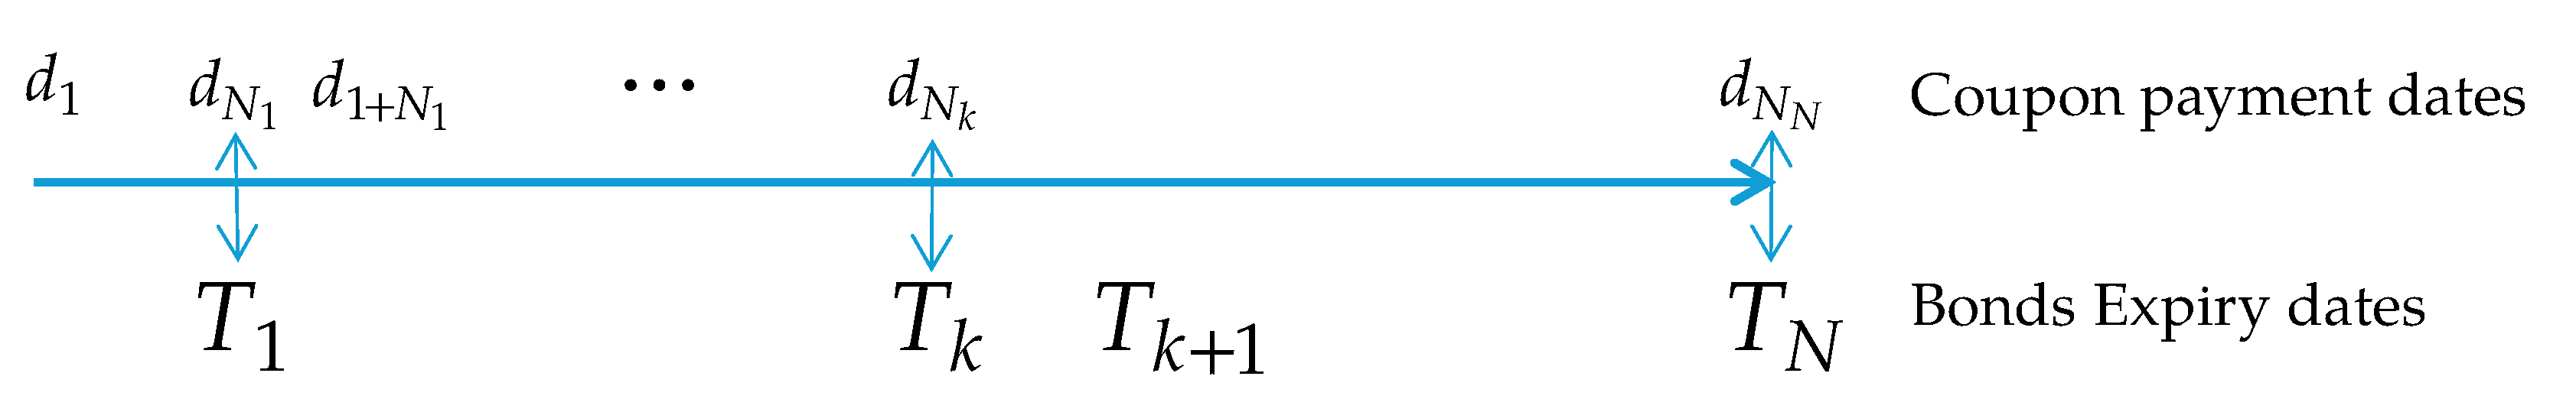
\includegraphics[width=0.8\textwidth]{Figure/note.pdf}
    \caption{Overlapping coupon payment dates for bootstrapping}\label{fig:payment-dates}
\end{figure}

For the $k$-th bond (with $N_k$ coupon dates up to $T_k$),
\begin{align*}
P(0, T_k) &= c_k \sum_{i=1}^{N_k} Z(0, d_i)\,\delta_i + Z(0, T_k), \\
\sum_{i=1}^{N_k} Z(0, d_i)\,\delta_i &= \frac{P(0, T_k) - Z(0, T_k)}{c_k}.
\end{align*}
Substituting this into the pricing equation for the $(k+1)$-th bond gives
\begin{align*}
P(0, T_{k+1}) &= c_{k+1} \sum_{i=1}^{N_{k+1}} Z(0, d_i)\,\delta_i + Z(0, T_{k+1}) \\
&= c_{k+1} \sum_{i=1}^{N_k} Z(0, d_i)\,\delta_i + c_{k+1} \sum_{i=1+N_k}^{N_{k+1}} Z(0, d_i)\,\delta_i + Z(0, T_{k+1}) \\
&= \frac{c_{k+1}}{c_k}\bigl[P(0, T_k) - Z(0, T_k)\bigr] + c_{k+1} \sum_{i=1+N_k}^{N_{k+1}} Z(0, d_i)\,\delta_i + Z(0, T_{k+1}).
\end{align*}
Only the last two terms depend on the unknown forward rate $\hat{y}_{k+1}$ over $(T_k, T_{k+1}]$, via
\[
c_{k+1} \sum_{i=1+N_k}^{N_{k+1}} Z(0, d_i)\,\delta_i + Z(0, T_{k+1})
= c_{k+1} \sum_{i=1+N_k}^{N_{k+1}} Z(0, T_k)(1 + \hat{y}_{k+1})^{-(d_i - T_k)}\,\delta_i + Z(0, T_k)(1 + \hat{y}_{k+1})^{-(T_{k+1} - T_k)}.
\]
This is a strictly decreasing equation in $\hat{y}_{k+1}$ (a polynomial in $(1 + \hat{y}_{k+1})^{-1}$ for equally spaced dates) and can be solved uniquely for $\hat{y}_{k+1}$ using standard root-finding methods such as Newton--Raphson.

\begin{example}[Two-Step Zero-Curve Bootstrapping]\label{ex:bootstrapping}
    Suppose the market quotes two single-curve OIS instruments with semi-annual day-count fractions $\delta_1 = \delta_2 = 0.5$:
    \begin{enumerate}
        \item A 6-month par deposit with simply compounded rate $r_{\mathrm{dep}} = 4.80\%$;
        \item A 1-year semi-annual par swap with fixed rate $s_{1\mathrm{Y}} = 5.00\%$.
    \end{enumerate}
    \textbf{Step 1: Extract $Z(0, 0.5)$.} A 6-month par deposit invests $\$1$ at $t = 0$ and returns $1 + \delta_1 r_{\mathrm{dep}}$ at $T_1 = 0.5$, so
    \[
    Z(0, 0.5) = \frac{1}{1 + 0.5 \times 0.0480} = \frac{1}{1.0240} = 0.97656250.
    \]
    \textbf{Step 2: Extract $Z(0, 1.0)$.} By the OIS par swap condition \eqref{eq:ois-par-rate}, the fixed leg equals the floating leg $1 - Z(0, 1.0)$:
    \[
    1 - Z(0, 1.0) = s_{1\mathrm{Y}}\bigl[\delta_1 Z(0, 0.5) + \delta_2 Z(0, 1.0)\bigr] = 0.0500\bigl[0.5\,Z(0, 0.5) + 0.5\,Z(0, 1.0)\bigr].
    \]
    Collecting terms in $Z(0, 1.0)$ gives
    \[
    Z(0, 1.0)\bigl(1 + 0.5 \times 0.0500\bigr) = 1 - 0.5 \times 0.0500 \times 0.97656250 = 0.97558594,
    \]
    and therefore
    \[
    Z(0, 1.0) = \frac{0.97558594}{1.0250} = 0.95179116.
    \]
    (As a verification, the fixed leg is $0.0500 \times 0.5 \times (0.97656250 + 0.95179116) = 0.04820884$, matching the floating leg $1 - 0.95179116 = 0.04820884$.)

    \textbf{Step 3: Implied forward rate.} The implied simply compounded 6-month forward rate over $[0.5, 1.0]$ is
    \[
    f(0; 0.5, 1.0) = \frac{1}{0.5}\left[\frac{Z(0, 0.5)}{Z(0, 1.0)} - 1\right] = 2\left(\frac{0.97656250}{0.95179116} - 1\right) = 0.05205205 \approx 5.2052\%,
    \]
    while the corresponding annually compounded forward rate is $\hat{y}_2 = \bigl(Z(0, 0.5)/Z(0, 1.0)\bigr)^{2} - 1 \approx 5.2729\%$. Because the swap curve is upward-sloping ($5.00\% > 4.80\%$), the forward rate over $[0.5, 1.0]$ lies above the 1-year par rate.
\end{example}

\section{Introduction to Credit Risk}

\subsection*{Credit Spreads}
\begin{definition}\label{def:survival-prob}
    Given a hazard rate (default intensity) function $\lambda(u) \geq 0$ for the time to default $\tau$, the \textbf{survival probability} from time $t$ to maturity $T$ is the probability that the issuer does not default by time $T$ (given survival to $t$):
    \[
    S(t, T) = \exp\!\left(-\int_t^T \lambda(u)\dd u\right).
    \]
\end{definition}

Let $B(0, T)$ be the price of a defaultable (credit-risky) zero-coupon bond. Because investors require compensation for default risk, its yield $\hat{y}'$ exceeds the risk-free yield $\hat{y}$:
\begin{align*}
Z(0, T) &= \exp\!\left(-\int_0^T \hat{y}(u)\dd u\right), \\
B(0, T) &= \exp\!\left(-\int_0^T \hat{y}'(u)\dd u\right) \\
&= \exp\!\left(-\int_0^T \bigl([\hat{y}'(u) - \hat{y}(u)] + \hat{y}(u)\bigr)\dd u\right) \\
&= \exp\!\left(-\int_0^T [\hat{y}'(u) - \hat{y}(u)]\dd u\right) Z(0, T) \\
&= \exp\!\left(-\int_0^T s(u)\dd u\right) Z(0, T),
\end{align*}
where $s(u) = \hat{y}'(u) - \hat{y}(u)$ is the \textbf{credit spread}.

Observe that $\exp(-\int_0^T s(u)\dd u)$ has the exact same form as the survival probability $S(0, T)$. Thus, under zero recovery, \textbf{a risky zero-coupon bond $B(0, T)$ equals a risk-free zero-coupon bond multiplied by the issuer's survival probability}, with the credit spread $s(t)$ playing the role of the hazard rate $\lambda(t)$.

Under the risk-neutral valuation framework, letting $\tau$ denote the random default time, we write
\[
B(0, T) = \E^{\Q}\!\left[e^{-\int_0^T r_s\dd s}\,\ind_{\tau > T}\right],
\]
where $\ind_{\tau > T}$ equals $1$ if default has not occurred by maturity $T$ and $0$ otherwise.

\subsection*{Credit Recovery}
In practice, bondholders typically recover a fraction $R \in [0, 1]$ of par value in the event of default. Assuming (i) independence between the default time $\tau$ and the risk-free short rate $r_s$, and (ii) the recovery-at-maturity convention (where $R$ is paid at $T$ if $\tau \leq T$), the risky zero-coupon bond price is
\begin{align*}
B(0, T) &= \E^{\Q}\!\left[e^{-\int_0^T r_s\dd s}\bigl(\ind_{\tau > T} + R\,\ind_{\tau \leq T}\bigr)\right] \\
&= \E^{\Q}\!\left[e^{-\int_0^T r_s\dd s}\bigl(\ind_{\tau > T}(1 - R) + R\bigr)\right] \\
&= \E^{\Q}\!\left[e^{-\int_0^T r_s\dd s}\right] \left(e^{-\int_0^T \lambda(s)\dd s}(1 - R) + R\right) \\
&\approx Z(0, T)\left(\left(1 - \int_0^T \lambda(s)\dd s\right)(1 - R) + R\right) \\
&= Z(0, T)\left(1 - \int_0^T (1 - R)\lambda(s)\dd s\right) \\
&\approx Z(0, T)\exp\!\left(-\int_0^T (1 - R)\lambda(s)\dd s\right).
\end{align*}
Thus, to first order, the credit spread is related to the hazard rate and recovery rate by the classic credit triangle approximation:
\[
s(t) \approx \lambda(t)(1 - R).
\]
As $R \to 1$, $s(t) \to 0$ because the investor suffers no loss upon default.

\subsection*{Credit Default Swaps}
\begin{definition}\label{def:cds}
    A \textbf{credit default swap} (CDS) is a bilateral derivative contract that allows an investor to \textbf{hedge or speculate} on the default risk of a reference entity. The protection buyer pays periodic premiums to the protection seller in exchange for a contingent payout if the reference entity defaults.
\end{definition}

A CDS consists of two legs on a stated notional (taken as $1$ below):
\begin{itemize}
    \item \textbf{Premium leg:} regular coupon payments made by the protection buyer until contract maturity $T_e$ or default $\tau$, whichever occurs first.
    \item \textbf{Protection leg:} a contingent payment of $(1 - R)$ made by the protection seller upon default (with $R = 40\%$ being a common market convention for senior unsecured corporate debt).
\end{itemize}

Let $Q_t = S(0, t) = \Prob^{\Q}(\tau > t)$ denote the time-$0$ survival curve of the reference entity (with $-\dd Q_s$ representing the risk-neutral probability of default in $[s, s+\dd s]$), and let $Z(0, s)$ be the risk-free discount curve over $[T_s, T_e]$, where $T_s$ and $T_e$ are the CDS start and maturity dates. Assuming the protection seller is default-free and default is independent of interest rates, let $T_s = T_0 < T_1 < \cdots < T_n = T_e$ be the regular premium payment dates.

The present value of the \textbf{protection leg} is
\begin{align*}
PV_{\text{prot}} &= -(1 - R)\int_{T_s}^{T_e} Z(0, s)\dd Q_s \\
&\approx -(1 - R)\sum_{i=1}^n Z(0, \bar{T}_i)\bigl[Q_{T_i} - Q_{T_{i-1}}\bigr],
\end{align*}
where $\bar{T}_i = \frac{T_i + T_{i-1}}{2}$ approximates the timing of a default in $[T_{i-1}, T_i]$ by the interval midpoint (note that $Q_{T_i} \leq Q_{T_{i-1}}$, so $-(Q_{T_i} - Q_{T_{i-1}}) \geq 0$).

For the \textbf{premium leg} with annualized spread $c$, consider the $i$-th coupon $P_i$ associated with accrual period $[T_{i-1}, T_i]$ and day-count fraction $\delta_i$. The full coupon $c\,\delta_i$ is paid at $T_i$ if $\tau > T_i$; if default occurs at $s \in [T_{i-1}, T_i]$, a pro-rata accrued premium $c\,\delta_i\frac{s - T_{i-1}}{T_i - T_{i-1}}$ is paid; if $\tau < T_{i-1}$, no payment is made. Thus
\[
P_i = c\,\delta_i Q_{T_i} Z(0, T_i) - c\,\delta_i \int_{T_{i-1}}^{T_i} \left(\frac{s - T_{i-1}}{T_i - T_{i-1}}\right) Z(0, s)\dd Q_s.
\]
Summing over all $n$ periods gives $\sum_{i=1}^n P_i$:
\[
PV_{\text{prem}} = \sum_{i=1}^n \left(c\,\delta_i Q_{T_i} Z(0, T_i) - c\,\delta_i \int_{T_{i-1}}^{T_i} \left(\frac{s - T_{i-1}}{T_i - T_{i-1}}\right) Z(0, s)\dd Q_s\right).
\]
For a protection buyer (payer CDS), the net present value is $PV_{\text{prot}} - PV_{\text{prem}}$, and the \textbf{par CDS spread} $c^*$ is the running rate $c$ that sets this value to zero. Writing $PV_{\text{prem}}(c) = c \cdot \mathrm{RPV01}$, where $\mathrm{RPV01}$ denotes the \textbf{risky annuity} (the present value of a unit running spread, including accrued premium upon default), we have $c^* = PV_{\text{prot}} / \mathrm{RPV01}$.

\paragraph{ISDA Big Bang Standardization.}
Following the \textbf{ISDA Big Bang Protocol (2009)}, single-name corporate CDS contracts no longer trade at par with bespoke running coupons. Instead, contracts carry a \textbf{standardized fixed running coupon} $c_{\mathrm{std}} \in \{100\text{ bps},\, 500\text{ bps}\}$ (typically $100\text{ bps}$ for investment-grade issuers and $500\text{ bps}$ for high-yield issuers) paid on standard quarterly IMM dates (March 20, June 20, September 20, December 20). The economic difference between the market par spread $c^*$ and the fixed coupon $c_{\mathrm{std}}$ is settled at inception through an \textbf{upfront payment} from the protection buyer to the seller:
\[
\mathrm{Upfront} = PV_{\text{prot}} - PV_{\text{prem}}(c_{\mathrm{std}}) = (c^* - c_{\mathrm{std}})\,\mathrm{RPV01}.
\]
Standardizing coupons makes offsetting CDS positions fungible and enables central clearing.

\begin{example}[1-Year Quarterly CDS Valuation and Par Spread]\label{ex:cds-valuation}
    Consider a 1-year CDS on a unit notional with quarterly payment dates $T_i = 0.25i$ ($i = 1, 2, 3, 4$, $\delta_i = 0.25$), a flat continuously compounded hazard rate $\lambda = 2\%$ (so $Q_t = e^{-0.02t}$ and $-\dd Q_s = \lambda e^{-\lambda s}\dd s$), recovery rate $R = 40\%$, and a flat continuously compounded risk-free rate $r = 4\%$ (so $Z(0, t) = e^{-0.04t}$).

    Table~\ref{tab:cds-example} tabulates the quarterly survival probabilities, discount factors, and default probabilities $-\Delta Q_i = Q_{T_{i-1}} - Q_{T_i}$ together with the midpoint discount factors $Z(0, \bar{T}_i)$ at $\bar{T}_i = (T_{i-1} + T_i)/2$.

    \begin{table}[!htbp]
        \centering
        \caption{Quarterly quantities for the 1-year CDS ($\lambda = 2\%$, $r = 4\%$, $R = 40\%$)}\label{tab:cds-example}
        \begin{tabular}{cccccc}
            \toprule
            $T_i$ & $Q_{T_i}$ & $Z(0, T_i)$ & $\bar{T}_i$ & $Z(0, \bar{T}_i)$ & $Q_{T_{i-1}} - Q_{T_i}$ \\
            \midrule
            $0.25$ & $0.995012$ & $0.990050$ & $0.125$ & $0.995012$ & $0.004988$ \\
            $0.50$ & $0.990050$ & $0.980199$ & $0.375$ & $0.985112$ & $0.004963$ \\
            $0.75$ & $0.985112$ & $0.970446$ & $0.625$ & $0.975310$ & $0.004938$ \\
            $1.00$ & $0.980199$ & $0.960789$ & $0.875$ & $0.965605$ & $0.004913$ \\
            \bottomrule
        \end{tabular}
    \end{table}

    \textbf{1. Protection leg.} Integrating analytically with $r + \lambda = 0.06$ gives the exact protection leg value
    \[
    PV_{\text{prot}} = (1 - R)\int_0^1 e^{-rs}\,\lambda e^{-\lambda s}\dd s = (1 - 0.40)\cdot\frac{0.02}{0.06}\bigl(1 - e^{-0.06}\bigr) = 0.01164709.
    \]
    (The discrete midpoint approximation $(1 - R)\sum_{i=1}^4 Z(0, \bar{T}_i)(Q_{T_{i-1}} - Q_{T_i}) = 0.01164700$ agrees to six decimal places.)

    \textbf{2. Premium leg (risky annuity $\mathrm{RPV01}$).} Setting $c = 1$, the scheduled quarterly payments contribute
    \[
    \mathrm{RPV01}_{\mathrm{sched}} = \sum_{i=1}^4 \delta_i\,Q_{T_i}\,Z(0, T_i) = 0.25\bigl(0.985112 + 0.970446 + 0.955997 + 0.941765\bigr) = 0.96332987.
    \]
    For the $\delta_i$-scaled accrued premium paid upon default in $[T_{i-1}, T_i]$, letting $k = r + \lambda = 0.06$, each interval contributes analytically
    \[
    \delta_i \int_{T_{i-1}}^{T_i} \frac{s - T_{i-1}}{T_i - T_{i-1}}\,e^{-rs}\,\lambda e^{-\lambda s}\dd s
    = \lambda\left[\frac{e^{-k T_{i-1}}}{k^2} - \left(\frac{\delta_i}{k} + \frac{1}{k^2}\right)e^{-k T_i}\right].
    \]
    Summing over $i = 1, \ldots, 4$ yields $\mathrm{RPV01}_{\mathrm{accr}} = 0.00242041$ (the midpoint approximation $\sum_{i=1}^4 \frac{\delta_i}{2} Z(0, \bar{T}_i)(Q_{T_{i-1}} - Q_{T_i}) = 0.00242646$). Combining both components gives
    \[
    \mathrm{RPV01} = \mathrm{RPV01}_{\mathrm{sched}} + \mathrm{RPV01}_{\mathrm{accr}} = 0.96332987 + 0.00242041 = 0.96575028.
    \]

    \textbf{3. Exact par CDS spread.} Dividing $PV_{\text{prot}}$ by $\mathrm{RPV01}$ gives
    \[
    c^* = \frac{0.01164709}{0.96575028} = 0.01206015 \approx 120.60\text{ bps},
    \]
    which closely matches the first-order credit triangle approximation $\lambda(1 - R) = 0.02 \times 0.60 = 120.00\text{ bps}$ (the slight $0.60\text{ bps}$ excess arises from discrete quarterly coupon payments compared with continuous protection). Under ISDA Big Bang conventions with $c_{\mathrm{std}} = 100\text{ bps}$, the protection buyer pays an upfront fee of $(0.01206015 - 0.01000000) \times 0.96575028 = 0.0019896$ (about $19.90\text{ bps}$ of notional).
\end{example}

\subsection*{Counterparty Credit Risk and Valuation Adjustments (XVA)}
All derivative pricing formulas derived earlier in this text assume that both counterparties are default-free and can fund positions at the risk-free rate. Following the 2008 financial crisis (highlighted by the default of Lehman Brothers), market practice and regulatory frameworks (Basel III) require adjusting the idealized risk-free value $V_0$ of an over-the-counter derivative for counterparty credit risk, own default risk, and funding costs. Collectively, these adjustments are known as \textbf{XVA} (valuation adjustments).

\paragraph{Derivation of Unilateral CVA.}
Consider an uncollateralized OTC derivative held by a default-free bank against a risky counterparty $C$, with maturity $T$ and risk-free mark-to-market value $V_t$ from the bank's perspective. Let $\tau_C$ be the counterparty's random default time, $Q_t^C = \Prob^{\Q}(\tau_C > t)$ its risk-neutral survival curve, and $R_C \in [0, 1]$ its recovery rate.

At the default time $\tau_C \leq T$, the close-out payoff is asymmetric:
\begin{itemize}
    \item If $V_{\tau_C} > 0$, the bank is a creditor owed $V_{\tau_C}$ but recovers only $R_C V_{\tau_C}$, suffering a loss of $(1 - R_C) V_{\tau_C}$.
    \item If $V_{\tau_C} \leq 0$, the bank still owes $|V_{\tau_C}|$ in full to the counterparty's estate, suffering zero credit loss.
\end{itemize}
Hence, the discounted loss suffered by the bank upon counterparty default is $D(\tau_C)(1 - R_C) V_{\tau_C}^+ \ind_{\tau_C \leq T}$, where $V_t^+ = \max(V_t, 0)$. The unilateral \textbf{Credit Valuation Adjustment (CVA)} is the risk-neutral expected discounted credit loss:
\[
\mathrm{CVA} = \E^{\Q}\!\left[D(\tau_C)(1 - R_C) V_{\tau_C}^+ \ind_{\tau_C \leq T} \;\middle|\; \F_0\right],
\]
so that the credit-adjusted value of the contract is $\widehat{V}_0 = V_0 - \mathrm{CVA}$.

Under the standard assumption that counterparty default $\tau_C$ is independent of market risk factors and interest rates (the absence of \textbf{wrong-way risk}), conditioning on $\tau_C = t$ with risk-neutral density $-\dd Q_t^C$ and factoring the expectation yields
\begin{equation}\label{eq:unilateral-cva}
\mathrm{CVA} = (1 - R_C)\int_0^T Z(0, t)\,\mathrm{EPE}(t)\,(-\dd Q_t^C),
\end{equation}
where $\mathrm{EPE}(t) = \E^{\Q}[V_t^+ \mid \F_0]$ (more generally, $\E^{\Prob^t}[V_t^+ \mid \F_0]$ under stochastic interest rates) is the \textbf{Expected Positive Exposure} at time $t$. Notice that CVA behaves like a strip of contingent options on the derivative's own mark-to-market value $V_t$: even a swap with $V_0 = 0$ at inception has strictly positive $\mathrm{EPE}(t)$ for $t > 0$ and therefore carries a nonzero CVA charge. When exposure $V_t^+$ and counterparty default probability are positively correlated (wrong-way risk), the factorization \eqref{eq:unilateral-cva} understates true credit risk and joint simulation of credit and market factors is required.

\paragraph{The Bilateral XVA Valuation Equation.}
In practice, both the bank $B$ and its counterparty $C$ can default, and uncollateralized derivative exposures must be financed at the bank's unsecured funding spread $s_F(t)$ over the risk-free OIS rate. Accounting for these effects yields the \textbf{bilateral XVA valuation equation}:
\begin{equation}\label{eq:xva-equation}
\widehat{V}_0 = V_0 - \mathrm{CVA} + \mathrm{DVA} - \mathrm{FVA},
\end{equation}
where:
\begin{itemize}
    \item \textbf{CVA (Credit Valuation Adjustment):} the expected discounted loss to the bank if counterparty $C$ defaults first ($\tau_C \leq T$ and $\tau_C < \tau_B$) while $V_{\tau_C} > 0$, reducing the contract value.
    \item \textbf{DVA (Debit Valuation Adjustment):} the symmetric adjustment for the bank's own default risk ($\tau_B \leq T$ and $\tau_B < \tau_C$) when the contract has negative mark-to-market value from the bank's perspective. In the unilateral approximation,
    \[
    \mathrm{DVA} = (1 - R_B)\int_0^T Z(0, t)\,\mathrm{ENE}(t)\,(-\dd Q_t^B),
    \]
    where $\mathrm{ENE}(t) = \E^{\Q}[(-V_t)^+ \mid \F_0]$ is the \textbf{Expected Negative Exposure}, $R_B$ is the bank's recovery rate, and $Q_t^B = \Prob^{\Q}(\tau_B > t)$ is the bank's survival curve. Because DVA makes both parties agree on the bilateral price ($\widehat{V}_0^B = -\widehat{V}_0^C$), it restores accounting symmetry, though hedging one's own default is notoriously difficult in practice.
    \item \textbf{FVA (Funding Valuation Adjustment):} the expected present value of the cost (or benefit) of funding uncollateralized exposures at the bank's unsecured funding spread $s_F(t)$ above OIS. Under symmetric borrowing and lending spreads,
    \[
    \mathrm{FVA} = \int_0^T Z(0, t)\,s_F(t)\,\E^{\Q}[V_t \mid \F_0]\,Q_t^B Q_t^C\dd t,
    \]
    which splits into a \textbf{Funding Cost Adjustment (FCA)} on positive exposures and a \textbf{Funding Benefit Adjustment (FBA)} on negative exposures.
\end{itemize}
Modern dealer desks also incorporate \textbf{MVA} (Margin Valuation Adjustment, the cost of funding initial margin posted to central counterparties or under bilateral uncleared margin rules) and \textbf{KVA} (Capital Valuation Adjustment, the cost of holding regulatory capital over the life of the trade). Because $\mathrm{EPE}(t)$ and $\mathrm{ENE}(t)$ must be computed across an entire netting set of derivatives simultaneously, XVA computation is one of the largest applications of Monte Carlo simulation (Appendix~\ref{ch:monte-carlo}) and American Monte Carlo regression in quantitative finance.
